% !TeX spellcheck = it_IT

\documentclass[xcolor={x11names}]{beamer}
\usetheme{Berkeley}
\setbeamercolor*{structure}{bg=DodgerBlue3!20,fg=DodgerBlue3}
\setbeamercolor*{sidebar}{use=structure,bg=structure.fg!68!black}
\setbeamercolor*{palette primary}{use=structure,fg=white,bg=structure.fg}
\setbeamercolor*{palette secondary}{use=structure,fg=white,bg=structure.fg!70}
\setbeamercolor*{palette tertiary}{use=structure,fg=white,bg=structure.fg!50!black}
\setbeamercolor*{palette quaternary}{fg=white,bg=black}
\setbeamercolor*{alerted text}{use=structure,fg={structure.fg>wheel,2,5}}
\usefonttheme{serif}
%\usefonttheme{structuresmallcapsserif} %forse un po' troppo pretenzioso

\usepackage[english,italian]{babel}
\usepackage{siunitx}
\usepackage{tikz}
\usepackage{pgfplots}
\usepackage{pgfplotstable}
\pgfplotsset{
	compat=newest,
	every tick label/.append style={font=\tiny},
	every node near coord/.append style={font=\scriptsize,color=black},
	label style={font=\small},
	legend style={font=\small}
}
\usepgfplotslibrary{ternary}
\usetikzlibrary{calc}
\usepackage{url}
\usepackage[export]{adjustbox}
\usepackage[font={footnotesize,color=darkgray},justification=centering]{caption}
\usepackage{calc}

\title{OpenLDAT}
\subtitle{Un sistema di misurazione di metriche di latenza dei display}
\author{Federico Dossena}
\date{Anno Accademico 2020/2021}

\newlength\leftsidebar
\newlength\rightsidebar
\makeatletter
\setlength\leftsidebar{\beamer@leftsidebar}
\setlength\rightsidebar{\beamer@rightsidebar}
\makeatother

\begin{document}

\setbeamertemplate{navigation symbols}{} %rimuovi i bottoni di navigazione in basso
\hoffset=-1\leftsidebar %rimuovi il bordo a sx per la sidebar
\begin{frame}[plain]
	\begin{minipage}{\textwidth+1\leftsidebar}
		\begin{center}
			
\includegraphics[width=0.6\textwidth]{Logo.png}\\
			\usebeamerfont{institute}{\bf Corso di Laurea Magistrale in Informatica}
		\end{center}
		\begin{beamercolorbox}[sep=12pt,center]{title}
			\usebeamerfont{title} \inserttitle\\
			\vspace{1mm}
			\usebeamerfont{subtitle} \insertsubtitle
		\end{beamercolorbox}
		\begin{center}
			\begin{minipage}[t]{0.45\textwidth}
				\begin{flushleft}
					\usebeamerfont{institute}
					{\bf Relatore:}\\
					Prof. Andrea TRENTINI\\
					\vspace{2mm}
					{\bf Correlatore:}\\
					Prof. Alessandro RIZZI
				\end{flushleft}
			\end{minipage}
			\begin{minipage}[t]{0.45\textwidth}
				\begin{flushright}
					\usebeamerfont{institute}
					{\bf Tesi di Laurea di:}\\
					Federico DOSSENA\\
					Matr. 909390
				\end{flushright}
			\end{minipage}
		\end{center}
		\vspace{3mm}
		\begin{center}
			\usebeamerfont{institute} \insertdate
		\end{center}
	\end{minipage}
\end{frame}

\setbeamertemplate{navigation symbols}{ %ripristina i pulsanti di navigazione in basso
	\hbox{
		\hbox{\insertslidenavigationsymbol}
		\hbox{\insertframenavigationsymbol}
		\hbox{\insertsubsectionnavigationsymbol}
		\hbox{\insertsectionnavigationsymbol}
		\hbox{\insertdocnavigationsymbol}
		\hbox{\insertbackfindforwardnavigationsymbol}
	}
}
\hoffset=0mm %ripristina il bordo a sx per la sidebar

\section{Introduzione}
\begin{frame}
	\frametitle{Cos'è OpenLDAT}
	\begin{itemize}
		\item Sistema automatico di \alert{misurazione di metriche di latenza dei display}
		\item Nato dall'esigenza di misurare la \alert{latenza totale di un sistema}
		\item \alert{Nessun dispositivo simile sul mercato}
		\item Progetto totalmente \alert{libero}
	\end{itemize}
\end{frame}

\section{Dispositivo}
\begin{frame}
	\frametitle{Dispositivo OpenLDAT (1)}
	\begin{columns}
		\column{0.5\textwidth}
		\begin{itemize}
			\item Microcontroller \alert{ATmega32U4}
			\item Fototransistor \alert{ALS-PT19}
		\end{itemize}
		\column{0.5\textwidth}
		\begin{itemize}
			\item \alert{PCB} personalizzato
			\item Comunicazione via USB
		\end{itemize}
	\end{columns}
	\begin{figure}
		\centering
		\adjincludegraphics[trim={{.10\width} 0 {.20\width} 0},clip,height=0.55\textheight]{Dispositivo_files/assembly_10.jpg}
		\adjincludegraphics[trim={{.12\width} 0 {.18\width} 0},clip,height=0.55\textheight]{Dispositivo_files/assembly_09.jpg}
	\end{figure}
\end{frame}
\begin{frame}
	\frametitle{Dispositivo OpenLDAT (2)}
	\begin{columns}
		\column{0.5\textwidth}
		\begin{itemize}
			\item \alert{Click autogenerati} o dall'esterno
			\item \alert{LED per validazione} dei risultati
		\end{itemize}
		\column{0.5\textwidth}
		\begin{itemize}
			\item \alert{Case stampabile}
			\item \alert{Poco costoso}
			\item Facile da realizzare
		\end{itemize}
	\end{columns}
	\begin{figure}
		\centering \adjincludegraphics[clip,height=0.65\textheight]{Dispositivo_files/assembly_15.jpg}
	\end{figure}
\end{frame}

\section{Applicazione}
\begin{frame}
	\frametitle{Applicazione OpenLDAT (1)}
	\begin{itemize}
        \item \alert{Applicazione grafica} per eseguire i test in modo semplice
        \item \alert{Multipiattaforma} (Windows, GNU/Linux, MacOS)
    \end{itemize}
	\begin{figure}
		\centering 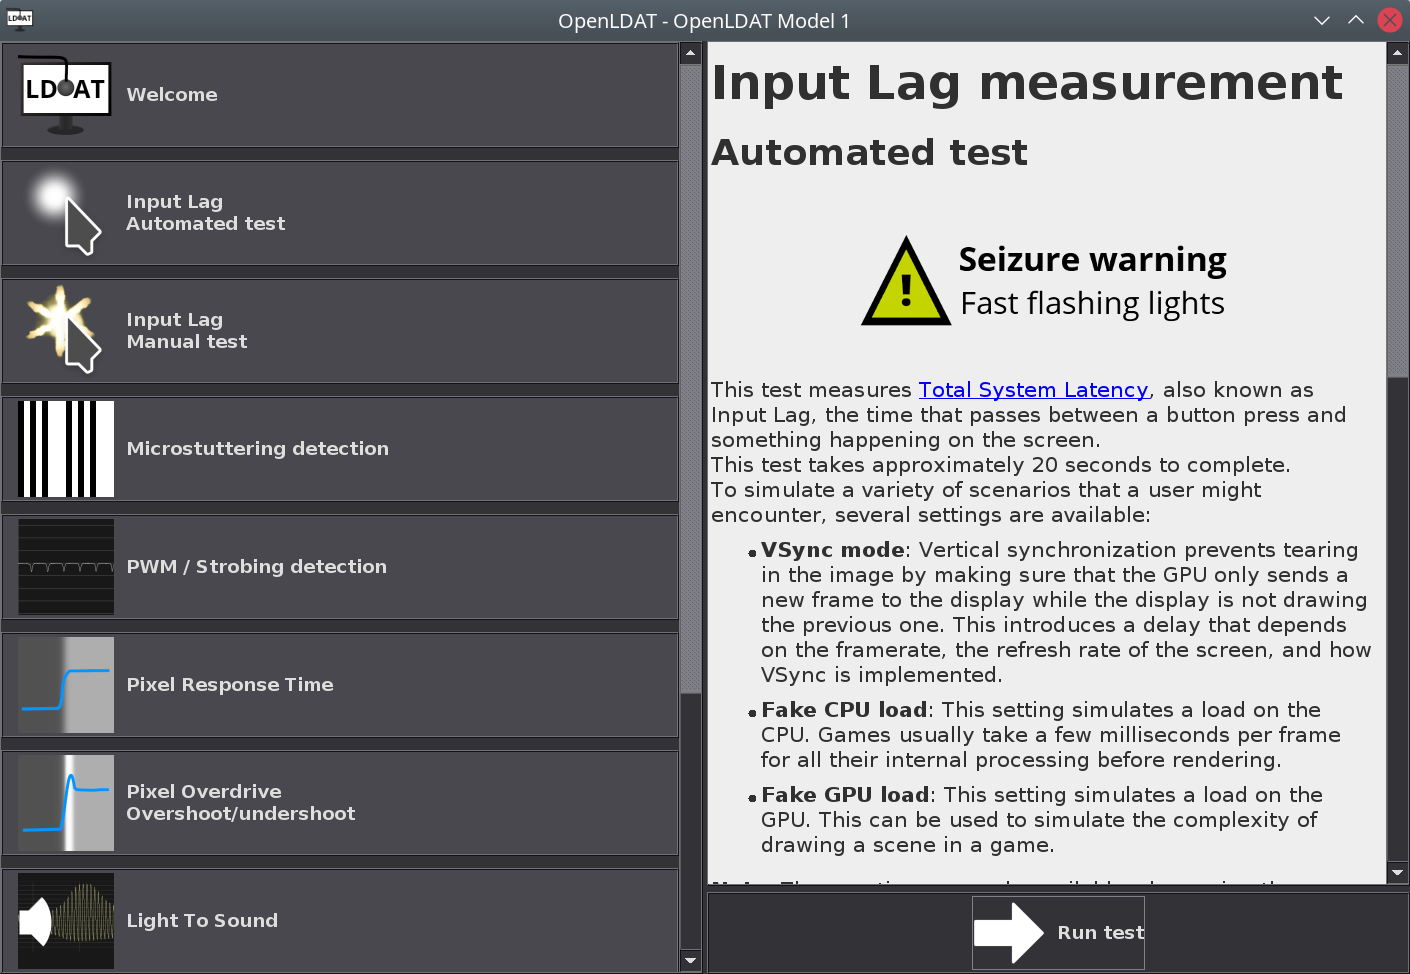
\includegraphics[height=0.7\textheight]{Applicazione_files/gui_mainMenu2.png}
	\end{figure}
\end{frame}
\begin{frame}
	\frametitle{Applicazione OpenLDAT (2)}
	Funzionalità: \begin{itemize}
		\item Misurazione automatica o interattiva della \alert{latenza totale del sistema}
		\item \alert{Rilevamento del microstuttering}
		\item \alert{Rilevamento di PWM e noise}
		\item \alert{Tempi di risposta dei pixel}
		\item \alert{Overdrive dei pixel}
		\item \alert{Light to Sound}
	\end{itemize}
\end{frame}
\begin{frame}[shrink=10]
	\frametitle{Applicazione OpenLDAT (3)}
	\begin{figure}
		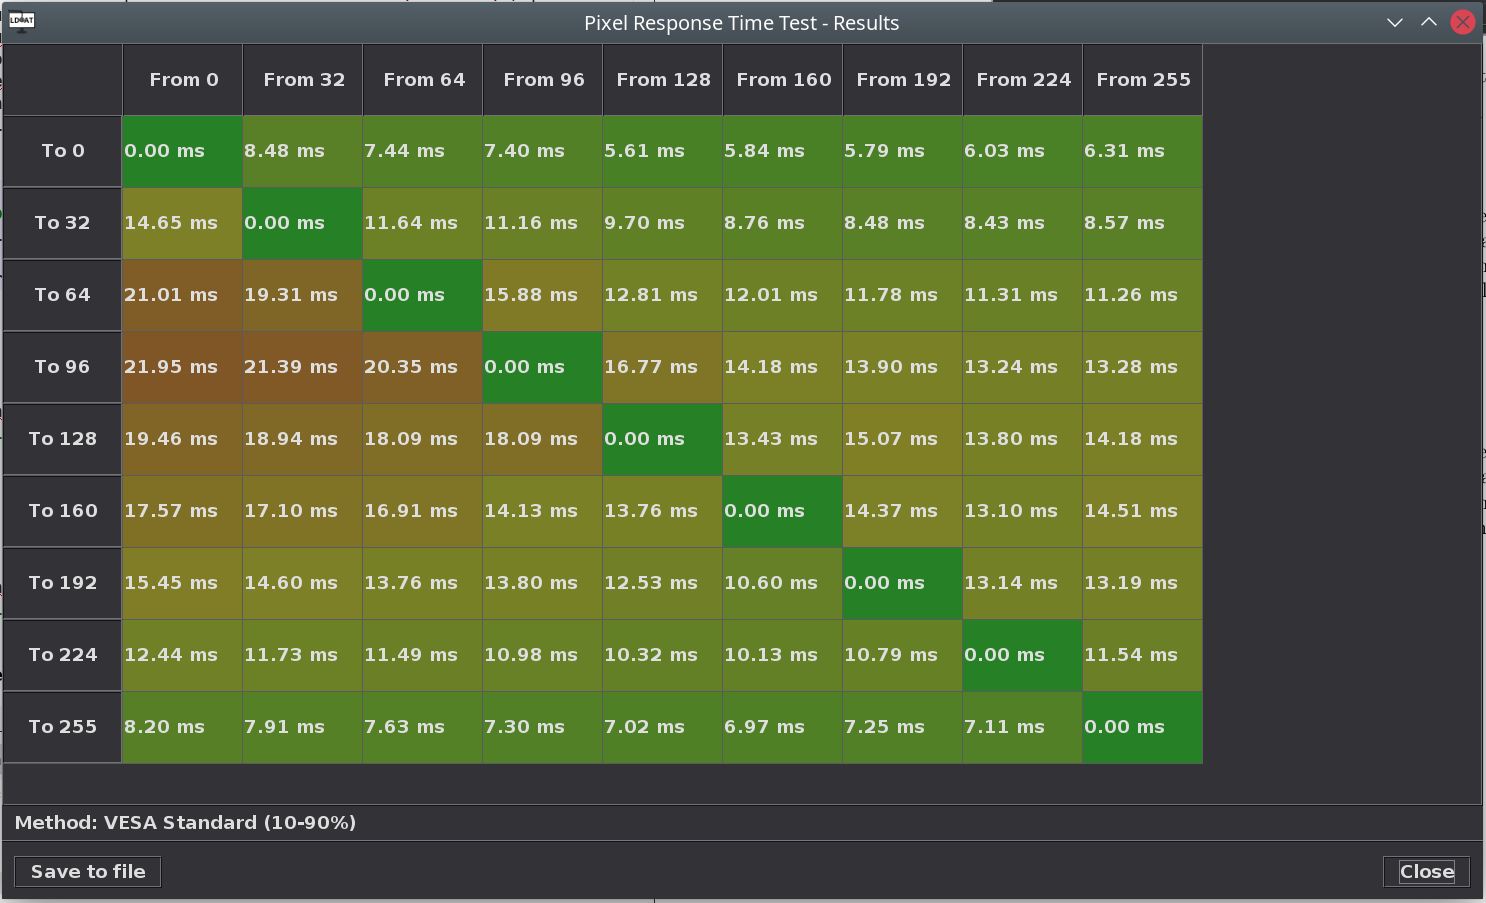
\includegraphics[width=\textwidth]{Applicazione_files/gui_pixelresponse_results.png}
		\caption*{Risultati di un test dei tempi di risposta dei pixel (AOC Q2770P)}
	\end{figure}
\end{frame}

\section{Risultati sperimentali}
\begin{frame}
	\frametitle{Risultati sperimentali}
	\begin{itemize}
		\item Testati \alert{oltre 20 display di tipi e periodi diversi}
		\item Modalità controllate
		\item \alert{Combinazioni hardware e software diverse}
		\item In fase di test sono emersi \alert{alcuni comportamenti interessanti}
		\item Sono stati selezionati alcuni test rappresentativi per questa presentazione
	\end{itemize}
\end{frame}
\begin{frame}[fragile,shrink=18]
	\frametitle{Input lag (1)}
	\begin{figure}
        \pgfplotstableread[col sep=comma]{
            model,novsync,vsync
            Acer Predator XB271HU (165Hz G-Sync),6.3,32.5
            Samsung C34H890 (100Hz Freesync),11.8,52.8
            ASUS VP228HE (60Hz),13.1,86.8
            LG E2360 (60Hz),14.1,89.6
            BenQ GL2706PQ (60Hz),27.7,93.7
            AOC Q2770P (60Hz),29.8,95.8
            Sharp LC-40FG3242E (60Hz TV),37.1,108.8
            Samsung P2770HD (60Hz TV),41.1,111.9
        }\dataset
        \begin{tikzpicture}
            \begin{axis}[xbar, bar width=8pt, y dir=reverse, ytick=data, yticklabels from table={\dataset}{model}, yticklabel style={text width=3cm, align=right}, table/y expr = \coordindex, nodes near coords, reverse legend, legend style={at={(7.25cm,-0.75cm)},anchor=east},xlabel=Ritardo (ms), width=9cm, height=8.25cm, xmin=0, ymin=-1, ymax=8, axis x line*=bottom, axis y line*=left] %ymax messo a mano con il numero di display per migliore formattazione
                \addplot table[x=vsync] {\dataset};
                \addplot table[x=novsync] {\dataset};
                \legend{VSync On, VSync Off}
            \end{axis}
        \end{tikzpicture}
        \caption*{Input lag di alcuni dei display testati}
    \end{figure}
\end{frame}
\begin{frame}[fragile,shrink=10]
	\frametitle{Input lag (2)}
	\begin{figure}
        \pgfplotstableread[col sep=comma]{
            config,novsync,vsync
            Linux Nvidia,28.0,69.1
            Windows Nvidia,28.4,95.3
            Linux AMD,28.7,86.1
            Windows AMD,29.6,93.9
            Windows Intel,31.3,103.4
            Linux Intel,34.1,86.6
            Linux Nouveau,44.3,86.0
        }\dataset
        \begin{tikzpicture}
            \begin{axis}[xbar, bar width=8pt, y dir=reverse, ytick=data, yticklabels from table={\dataset}{config}, yticklabel style={text width=1cm, align=right}, table/y expr = \coordindex, nodes near coords, reverse legend, legend style={at={(7.25cm,-0.75cm)},anchor=east}, xlabel=Ritardo (ms), width=8.5cm, height=7.5cm, ymin=-1, ymax=7,xmax=110, axis x line*=bottom, axis y line*=left]
                \addplot table[x=vsync] {\dataset};
                \addplot table[x=novsync] {\dataset};
                \legend{VSync On, VSync Off}
            \end{axis}
        \end{tikzpicture}
        \caption*{Input lag con combinazioni hardware/software diverse}
    \end{figure}
\end{frame}
\begin{frame}[fragile,shrink=10]
	\frametitle{Input lag (3)}
	\begin{figure}
        \pgfplotstableread[col sep=comma]{
            app,lag,emin,emax
            Mass Effect Legendary Ed. (2021),45.7,8.4,7.7
            Crysis (2007),51.9,6.7,8.6
            Doom Eternal (2020),52.8,4.6,2.4
            Unreal Tournament 2004 (2003),81.3,11.8,18.7
            Google Stadia 1080p60 (FTTH),121.4,34.4,119.6
            YouTube (Chromium),147.2,13.0,17.2
            Doom (1993),158.9,16.9,14.2
            Crysis Remastered (2020),182.5,17.8,23.5
        }\dataset
        \begin{tikzpicture}
            \begin{axis}[xbar, bar width=10pt, y dir=reverse, ytick=data, yticklabels from table={\dataset}{app}, yticklabel style={text width=4cm, align=right}, table/y expr = \coordindex, nodes near coords, xlabel=Ritardo (ms), width=8cm, height=7.5cm, ymin=-1, ymax=8, axis x line*=bottom, axis y line*=left] %ymax messo a mano con il numero di test per migliore formattazione
                \addplot[fill=gray, error bars/.cd, x dir = both, x explicit] table[x=lag, x error plus=emax, x error minus=emin] {\dataset};
            \end{axis}
        \end{tikzpicture}
        \caption*{Input lag di alcune applicazioni}
    \end{figure}
\end{frame}
\begin{frame}[fragile,shrink=20]
	\frametitle{Tempi di risposta dei pixel e overdrive}
	\begin{minipage}[c][\paperheight][c]{\textwidth}
		\begin{minipage}{0.57\textwidth}
			\begin{figure}
				\centering
				\pgfplotstableread[col sep=comma]{
					model,odoff,odoffemin,odoffemax,odon,odonemin,odonemax,fix
					BenQ XL2420T (TN),NaN,NaN,NaN,2.61,1.48,3.80,-10
					Samsung C34H890 (VA),7.81,5.17,27.90,7.79,4.26,18.25,-10
					LG 27GL850-B (IPS HDR),9.74,3.94,4.46,2.91,1.92,11.69,-10
					AOC Q2770P (IPS),12.33,6.06,9.01,7.37,3.09,3.74,-10
					Octigen M19W (TN),14.61,13.10,13.03,NaN,NaN,NaN,-10
					MacBook Pro 13" 2017 (IPS),19.49,8.74,12.60,NaN,NaN,NaN,-10
				}\dataset
				\begin{tikzpicture}
					\begin{axis}[xbar, bar width=8pt, y dir=reverse, ytick=data, yticklabels from table={\dataset}{model}, yticklabel style={text width=2cm, align=right}, table/y expr = \coordindex, nodes near coords, reverse legend, xlabel=Tempo di risposta (ms), width=6.25cm, height=7cm, xmin=0, ymin=-1, ymax=6, axis x line*=bottom, axis y line*=left] %ymax messo a mano con il numero di display per migliore formattazione
						\addplot plot[forget plot] table[x=fix] {\dataset};
						\addplot plot [error bars/.cd, x dir = both, x explicit] table[x=odoff, x error plus=odoffemax, x error minus=odoffemin] {\dataset};
						\addplot plot [error bars/.cd, x dir = both, x explicit] table[x=odon, x error plus=odonemax, x error minus=odonemin] {\dataset};
						%\legend{Overdrive Off, Overdrive On}
					\end{axis}
				\end{tikzpicture}
			\end{figure}
		\end{minipage}
		\begin{minipage}{0.33\textwidth}
			\begin{figure}
				\centering
				\pgfplotstableread[col sep=comma]{
					model,odoff,odoffemin,odoffemax,odon,odonemin,odonemax,fix
					,NaN,NaN,NaN,2.80,2.56,14.55,-10
					,0.32,0.32,1.79,1.21,1.21,6.43,-10
					,0.39,0.39,0.22,26.39,24.82,22.98,-10
					,0.17,0.17,0.41,4.14,4.14,16.32,-10
					,0.25,0.25,0.65,NaN,NaN,NaN,-10
					,0.22,0.22,0.59,NaN,NaN,NaN,-10
				}\dataset
				\begin{tikzpicture}
					\begin{axis}[xbar, bar width=8pt, y dir=reverse, ytick=data, yticklabels from table={\dataset}{model}, yticklabel style={text width=0cm, align=right}, table/y expr = \coordindex, nodes near coords, reverse legend, xlabel=Errore di transizione (\%), width=6.25cm, height=7cm, xmin=0, ymin=-1, ymax=6, axis x line*=bottom, axis y line*=left, legend style={at={(5.75cm,-0.75cm)},anchor=east}] %ymax messo a mano con il numero di display per migliore formattazione]
						\addplot plot[forget plot] table[x=fix] {\dataset};
						\addplot plot [error bars/.cd, x dir = both, x explicit] table[x=odoff, x error plus=odoffemax, x error minus=odoffemin] {\dataset};
						\addplot plot [error bars/.cd, x dir = both, x explicit] table[x=odon, x error plus=odonemax, x error minus=odonemin] {\dataset};
						\legend{Overdrive Off, Overdrive On}
					\end{axis}
				\end{tikzpicture}
			\end{figure}
		\end{minipage}
	\end{minipage}
\end{frame}
\begin{frame}
	\frametitle{Altri test}
	\begin{itemize}
		\setlength\itemsep{4mm}
		\item PWM e noise: \begin{itemize}
			\item \alert{Retroilluminazione PWM trovata solo su TV e display di fascia bassa}
			\item Nessuno dei display testati ha mostrato rumore
			\item \alert{Su alcuni display è rilevabile il ciclo di refresh dei pixel}
		\end{itemize}
		\item Microstuttering: \begin{itemize}
			\item \alert{Nessun display ha mostrato microstuttering a refresh rate nativo}
			\item Alcuni dei display hanno mostrato microstuttering in overclock
		\end{itemize}
	\end{itemize}
\end{frame}

\section{Conclusioni}
\begin{frame}
	\frametitle{Sviluppi futuri}
	\begin{itemize}
        \item Implementazione di \alert{altri backend grafici} nell'applicazione
        \item Migliorie all'hardware e all'applicazione per poter implementare \alert{altri test}
        \item Porting dell'applicazione su Android
        \item \alert{Commercializzazione del dispositivo}
        \item Realizzazione di un sito dove gli utenti possono postare i risultati
	\end{itemize}
\end{frame}
\begin{frame}
	\frametitle{Grazie per l'attenzione}
	\centering
	Per maggiori informazioni:\\
	\alert{\url{https://openldat.fdossena.com}}
\end{frame}

\end{document}
